\documentclass{SPANISH_acm_proc_article-sp}
\usepackage[latin1]{inputenc}
\hyphenation{a-le-a-to-ri-os o-pe-ra-dor in-di-vi-duos o-pe-ra-do-res re-pre-sen-ta-do pue-de va-lo-res re-pre-sen-ta-cio-nes a-na-li-za Con-ti-nen-tal co-rres-pon-dien-te ob-ten-cio\'on pro-ba-bi-li-dad}
\begin{document}

\title{Visitando la Plataforma Continental Argentina}
\subtitle{}

\numberofauthors{5}

\author
{
	%1st author
	\alignauthor
    Gustavo Maldonado \\
	\affaddr{Instituto Tecnol\'ogico de Buenos Aires (ITBA)} \\
	\affaddr{Buenos Aires, Argentina}\\
	\email{gmaldona@alu.itba.edu.ar}
	%2nd author
	\alignauthor
	Guido Marucci Blas \\
    \affaddr{Instituto Tecnol\'ogico de Buenos Aires (ITBA)} \\
	\affaddr{Buenos Aires, Argentina}\\
	\email{gmarucci@alu.itba.edu.ar}
	%3rd author
	\alignauthor	
    Santiago Perez De Rosso \\
    \affaddr{Instituto Tecnol\'ogico de Buenos Aires (ITBA)} \\
	\affaddr{Buenos Aires, Argentina}\\
	\email{sperezde@alu.itba.edu.ar}
	\and
	%4th author
	\alignauthor
	Nicolas Purita \\
    \affaddr{Instituto Tecnol\'ogico de Buenos Aires (ITBA)} \\
	\affaddr{Buenos Aires, Argentina}\\
	\email{npurita@alu.itba.edu.ar}	
	\and
    %5th author
    \alignauthor
    Luciano Zemin \\
    \affaddr{Instituto Tecnol\'ogico de Buenos Aires (ITBA)} \\
	\affaddr{Buenos Aires, Argentina}\\
	\email{lzemin@alu.itba.edu.ar}
}

\maketitle

\section*{RESUMEN}
En este art\'iculo se analiza el generador de n\'umeros aleatorios utilizado por la librer\'ia estandar de Java, per\'iodo de evoluci\'on y su funci\'on densidad de probabilidad de un \emph{modelo ecol\'ogico presa - predador} a partir de una muestra inicial y de las caracter\'isticas evolutivas del sistema (sus \emph{par\'ametros bi\'oticos}).
En particular, se analiza el caso de la zona sobre la Plataforma Continental Argentina
donde la especie \textit{Tibur\'on Pintarrojo} preda a la especie \textit{Salm\'on de Mar},
siendo esta \'ultima un importante recurso econ\'omico pesquero nacional.

\section*{Palabras Clave}
Modelo de \textit{Lokta-Volterra-Ancona}, \textit{Montecarlo}, \textit{Salm\'on de Mar},
\textit{Tibur\'on Pintarrojo}

\section{INTRODUCCI\'ON}
Es de una gran importancia econ\'omica aparte de biol\'ogica el estudio de la din\'amica
presa-predador de ciertas especies de recurso econ\'omico pesquero. En el presente art\'iculo
se analiza en particular el caso de la zona sobre la Plataforma Continental Argentina donde
la especie \emph{Salm\'on de Mar (Pseudopercis semifasciata)} es capturada desde una
latitud correspondiente a la desembocadura del R\'io Colorado, hasta el Golfo de San Juli\'an.
El \emph{Tibur\'on Pintarrojo (Haleaeulurus bivius)} es una de las cincuenta especies que
habitan la Plataforma Continental Argentina. Dicha especie preda al Salm\'on de Mar.
Ambas poblaciones est\'an en equilibrio din\'amico, pero no se tiene la suficiente 
cantidad de datos para estimar el ciclo poblacional del recurso, en este caso, el salm\'on.
El conocimiento de dicho ciclo, el cual constituye el per\'iodo de variaci\'on poblacional,
es un par\'ametro de fundamental importancia econ\'omica adem\'as de biol\'ogica. Ya que
este permite estimar los periodos de vedas o disminuci\'on de las tazas de captura
econ\'omica.

En la secci\'on \ref{sec:modelo} se presenta el modelo utilizado a lo largo del art\'iculo,
en la secci\'on \ref{sec:estimacion} se detalla el proceso de obtenci\'on de la
estimaci\'on de la funci\'on densidad de probabilidad del \emph{Per\'iodo}. Finalmente,
en la secci\'on \ref{sec:resultados} se presentan los resultados obtenidos y las
conclusiones finales.

\section{Generaci\'on de N\'umeros aleatorios}
A continuaci\'on se analiza el generador de n\'umeros aleatorios que usa la librer\'ia est\'andar
de Java en el m\'etodo \textit{nextDouble} en la clase java.util.Random. La implementaci\'on de dicho 
algoritmo est\'a basado en un generador de n\'umeros aleatorios congruencial lineal (GCL) con per\'iodo
de longitud $2^{48}$. Cada salida del generador se construye de la siguiente forma:

\begin{eqnarray}
	x_{i + 1} & = & (25214903917x_{i} + 11) \quad mod \  2^{48} \\
	u_{i} & = & x_{i} / 2^{48}
\end{eqnarray}

Para el an\'alisis del GCL se utiliza la semilla $s_{0} = 1320005715$ y se generan $n = 10000$ n\'umeros pseudo-aleatorios sin reiniciar el generador. En la figura (\ref{fig:histRandom}) se muestra un histograma con la frecuencia de aparici\'on de los n\'umeros pseudo-aleatorio los cuales fueron agrupados en 10 intervalos de clase. . En la figura (\ref{fig:random2D}) se muestra la representaci\'on de los pares $(u_{i}, u_{i+1})$ y en la figura (\ref{fig:random3D}) las ternas $(u_{1}, u_{i+1}, u_{i+2})$. 

\begin{figure}
\centering
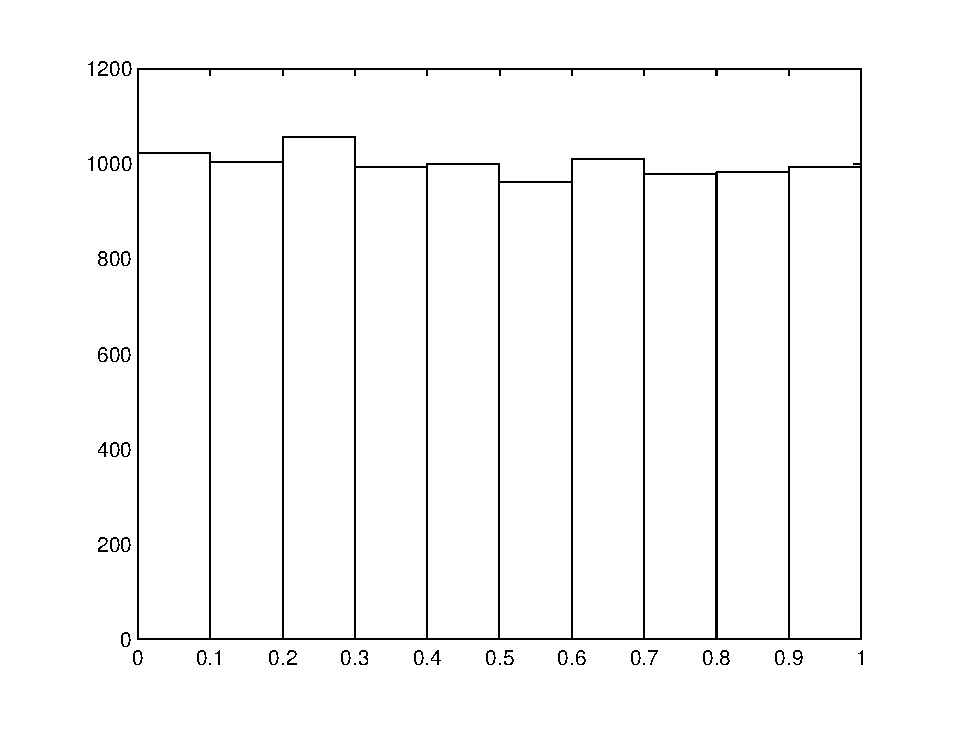
\epsfig{file=histRandom.eps, scale=0.55}
\caption{Frecuencia de aparici\'on de los n\'umeros pseudo-aleatorio}
\label{fig:histRandom}
\end{figure}

\begin{figure}
\centering
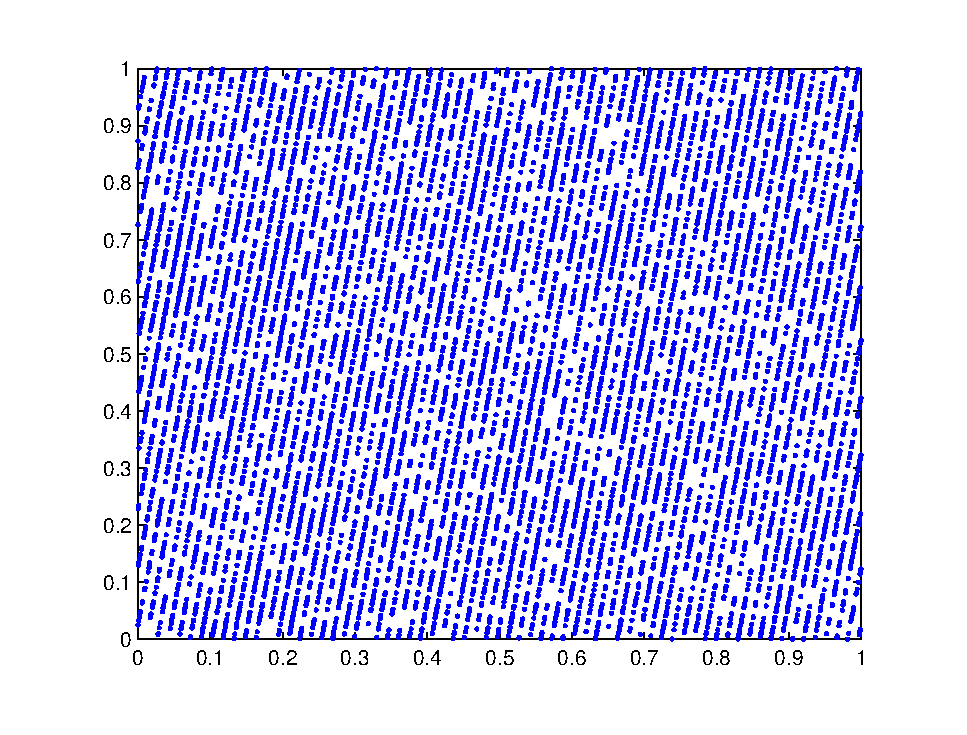
\epsfig{file=randomize2D.eps, scale=0.55}
\caption{Representaci\'on de los pares $(u_{i}, u_{i+1})$}
\label{fig:random2D}
\end{figure}

\begin{figure}
\centering
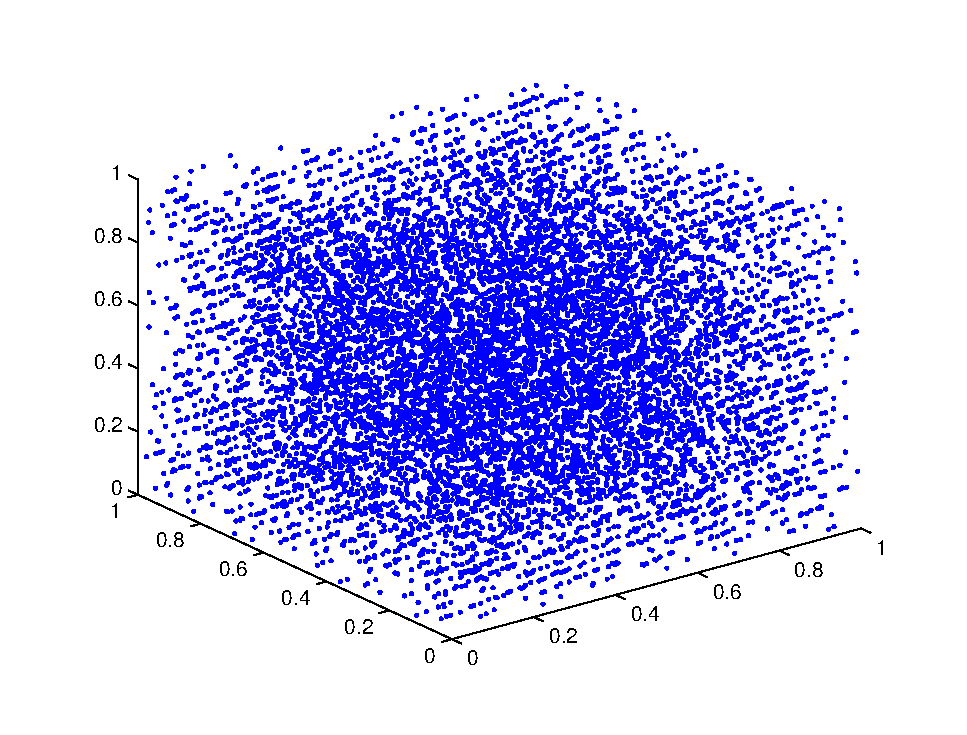
\epsfig{file=randomize3D.eps, scale=0.55}
\caption{Ternas $(u_{1}, u_{i+1}, u_{i+2})$}
\label{fig:random3D}
\end{figure}

Al observar las figuras \ref{fig:histRandom}, \ref{fig:random2D} y \ref{fig:random3D} se desea ver que la hip\'otesis, los n\'umeros pseudo-aleatorio generador por el GCL est\'an uniformemente distribuidos, no es rechazada. Para esto se realizan las pruebas de \textbf{Kolmogorov-Smirnov} y \textbf{Chi Cuadrado}.

\subsection{Kolmogorov-Smirnov}
Se realiza la prueba de Kolmogorov-Smirnov con un nivel de significaci\'on $\alpha = 0.05$ y 10 intervalos de clase. Para estos valores el valor cr\'itico es $D_{\alpha} = 0,4092$. La hip\'otesis a ver que no es rechazada es 

\begin{equation}
		H_{0}: D < D_{\alpha}
\end{equation}

Los n\'umeros generados por el GCL tienen una distribuci\'on uniforme. Usando la semilla $s_{0}$ para generar los $n$ n\'umeros aleatorios el c\'omputo del estad\'istico es $D = 0.100$. Entonces la hip\'otesis $H_{0}$ no es rechazada. 

\subsection{Chi-Cuadrado}
Se realiza la prueba de Chi-Cuadrado con un nivel de sinificaci\'on $\alpha = 0.05$, 10 intervalos de clase y 9 grados de libertad. Para estos valores el valor cr\'itico es $\chi_{n-1, \alpha} = 16.92$. La hip\'otesis a ver que no es rechazada es 

\begin{equation}
		H_{1}: \chi^2 < \chi^2_{n - 1, \alpha}
\end{equation}

Como el c\'omputo del estad\'istico es $\chi^2_{0} = 6.088000$, entonces las hip\'otesis $H_{1}$ no es rechazada.

\section{Modelizaci\'on del sistema}
\label{sec:modelo}
El sistema se modela utilizando el modelo de \textit{Lokta-Volterra-Ancona}. Se considera que el predador
se alimenta exclusivamente de la presa, mientras que esta \'ultima se alimenta de recursos ilimitados
que se encuentran en su h\'abitat. El ambiente no influye sobre el sistema, asi como el sexo o
el estado de salud de los individuos.\\
En las ecuaciones \ref{eq:modelo1} y \ref{eq:modelo2} se puede ver el modelo resultante:
\begin{equation}
\label{eq:modelo1}
\dot{x} = \lambda x - axy
\end{equation}
\begin{equation}
\label{eq:modelo2}
\dot{y} = bxy - \mu y
\end{equation}
donde $x(y)$ e $y(t)$ representan las poblaciones de la especie presa y predador, 
respectivamente. Las constantes $\lambda$, $\mu$ representan las tasa de crecimiento
poblacional de presas y predadores respectivamente, en ausencia de sus contrapartes.
Las constantes positivas $a$ y $b$ representan las tasas de encuentros perjudiciales para 
las presas y beneficiosos para predadores.\\


\section{Estimaci\'on de la funci\'on densidad de probabilidad del Per\'iodo}
\label{sec:estimacion}

Con el objetivo de estimar la funci\'on densidad de probabilidad del \emph{Per\'iodo}
se utiliza el m\'etodo de \textit{Monte Carlo}. El m\'etodo de \textit{Monte Carlo} es una metodolog\'ia
para obtener, mediante simulaci\'on, una muestra estad\'istica y computar estimadores
de par\'ametros para poblaciones mayores \textit{(Diaz, 2011)}. Las simulaciones fueron
realizadas con \textit{Matlab}. Para la resoluci\'on de las ecuaciones diferenciales se
 utiliza \textit{ODE45} que es el recomendado en
\textit{Matlab},est\'a basado en la f\'ormula expl\'icita de Runge-Kutta (4, 5) Dormand-Prince. Utiliza seis
funciones de valuaci\'on para calcular soluciones de precisi\'on de 4to y 5to orden. Este m\'etodo se considera
adaptativo ya que var\'ia el tama\~no de paso de acuerdo al error \textit{(Mathworks, 2011)}.

Asumiendo un valor estimado de $ \hat b = 0.0035 \, $a\~nos$^{-1} $ y suponiendo que
\begin{itemize}
\item $ a = (0.02 \, \underline{+} \, 0.001) \, $a\~nos$^{-1}$ uniformemente distribuida.
\item $ \lambda = \mathcal{N}(1.5 \, $a\~nos$^{-1}, 0.10) $ es una funci\'on de distribuci\'on de probabilidad normal de media
\item  $ \mu = \mathcal{N}(1.2 \, $a\~nos$^{-1}, 0.05) $ es una funci\'on de distribuci\'on de probabilidad normal de media $ 1.2$, a\~nos$^{-1}$ con un desv\'io lineal porcentual de $5\%$ 
\end{itemize}
se estima la funci\'on densidad de probabilidad del \emph{Per\'iodo}. El resultado obtenido al correr
15434 simulaciones se puede ver en la Figura (\ref{fig:histo}) en la cual se deduce que la funci\'on densidad de probabilidad se aproxima a una funci\'on de distribuci\'on $\mathcal{N}(5.87$a\~nos$^{-1}, 0.19)$ con un desv\'io est\'andar del 0.19\%.\\

En la figura (\ref{fig:presa}), la cual muestra el tama\~no de la poblaci\'on de la presa a lo largo de los a\~nos, se puede verificar que el per\'iodo se aproxima a \textit{6}.
\\
A partir del resultado obtenido se estima la probabilidad de que el peri\'odo del ciclo
poblacional sea menor o igual que 1, 5, 10 y 15 a\~nos obteniendo como resultado lo que se expresa en la tabla (\ref{fig:tableCycle}).


\begin{table}
\begin{tabular}{|c|c|c|}
	\hline
	A\~nos (Y) 	& 		X*		&		Probabilidad( P(X* $\leq$ Y)		\\
	\hline \hline
	1				&	-2563.5263	&	0 \\
	\hline
	5				&		-458.2631 & 0 \\
	\hline
	10		&	2173.3158 & 1 \\
	\hline
	15		& 4804.8947 & 1 \\
	\hline
\end{tabular}
	\caption{Estimaciones de probabilidad del ciclo poblacional}
	\label{fig:tableCycle}
\end{table}

\begin{figure}
\centering
\label{fig:histo}
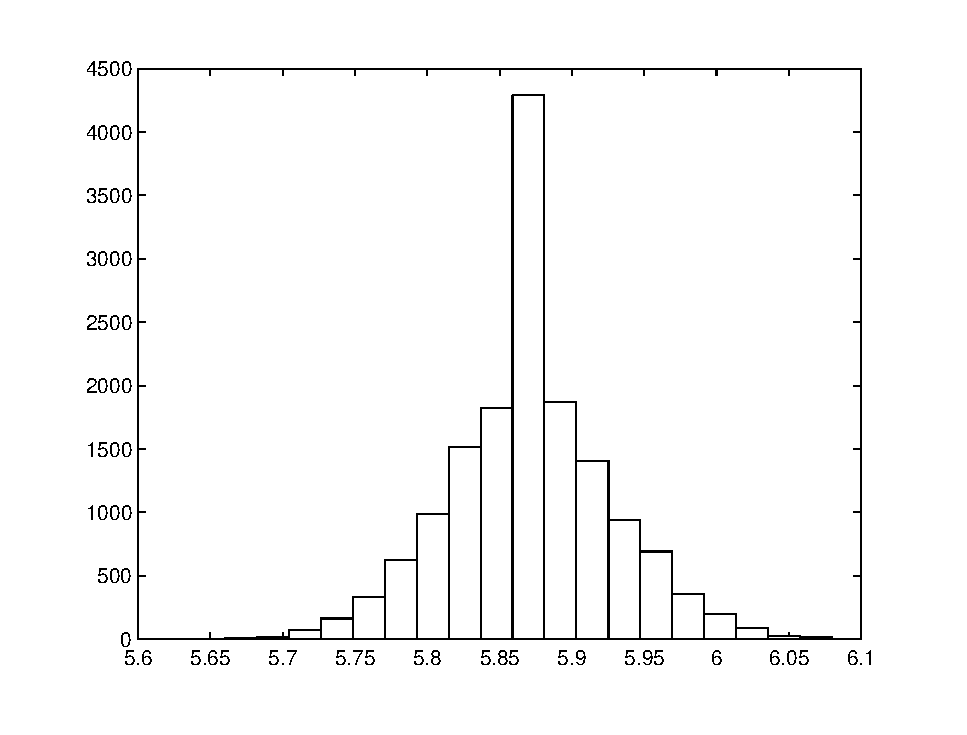
\epsfig{file=histPosta.eps, scale=0.4}
\caption{Funci\'on densidad de probabilidad del per\'iodo. Cantidad de ocurrencias versus per\'iodo.}
\end{figure}

\begin{figure}
\centering
\label{fig:presa}
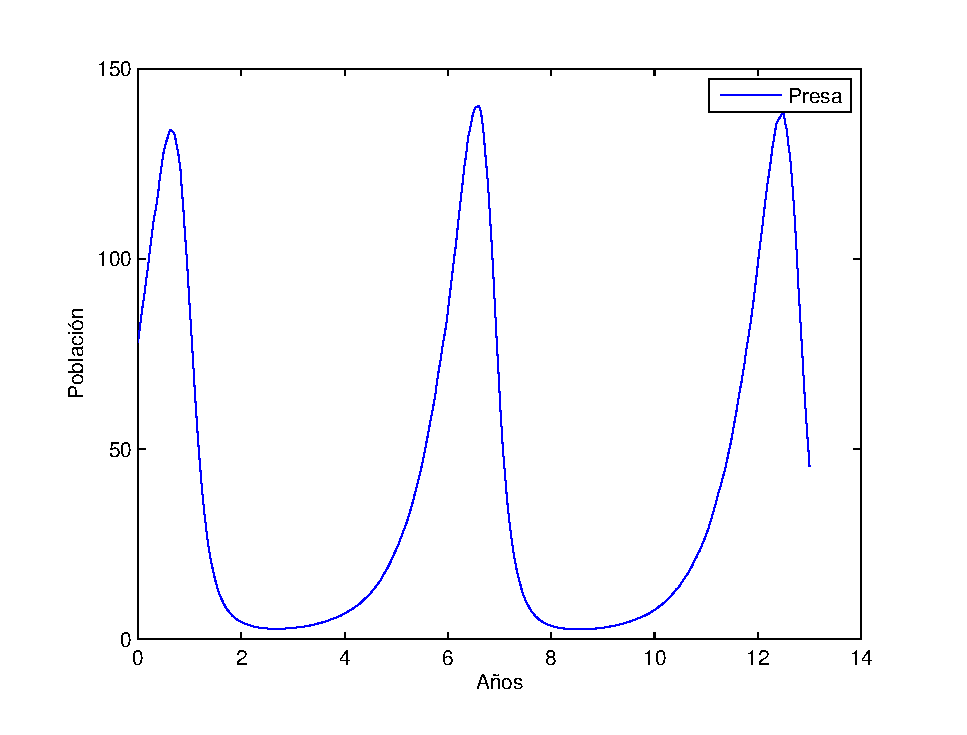
\epsfig{file=presa.eps, scale=0.4}
\caption{Tama\~no de la poblaci\'on de la presa en funci\'on del tiempo}
\end{figure}

\section{Modificaci\'on de una funci\'on de distribuci\'on }
Se cambia la distribuci\'on de uno de los par\'ametros que representan las interacciones entre las dos espcecies.
 El par\'ametro en cuesti\'on es $\mu$ y se le asigna una funci\'on de distribuci\'on triangular $\mathcal{T}(0,2,1)$.
 Se estima la funci\'on de densidad de probabilidad del \emph{Per\'iodo} utilizando un histograma que es una herramienta provista estad\'istica descriptiva. 
 \\
 La figura (\ref{fig:histoTriangulo}) es el resultado obtenido luego de correr 5772 simulaciones para obtener el per\'iodo.


\begin{figure}
\centering
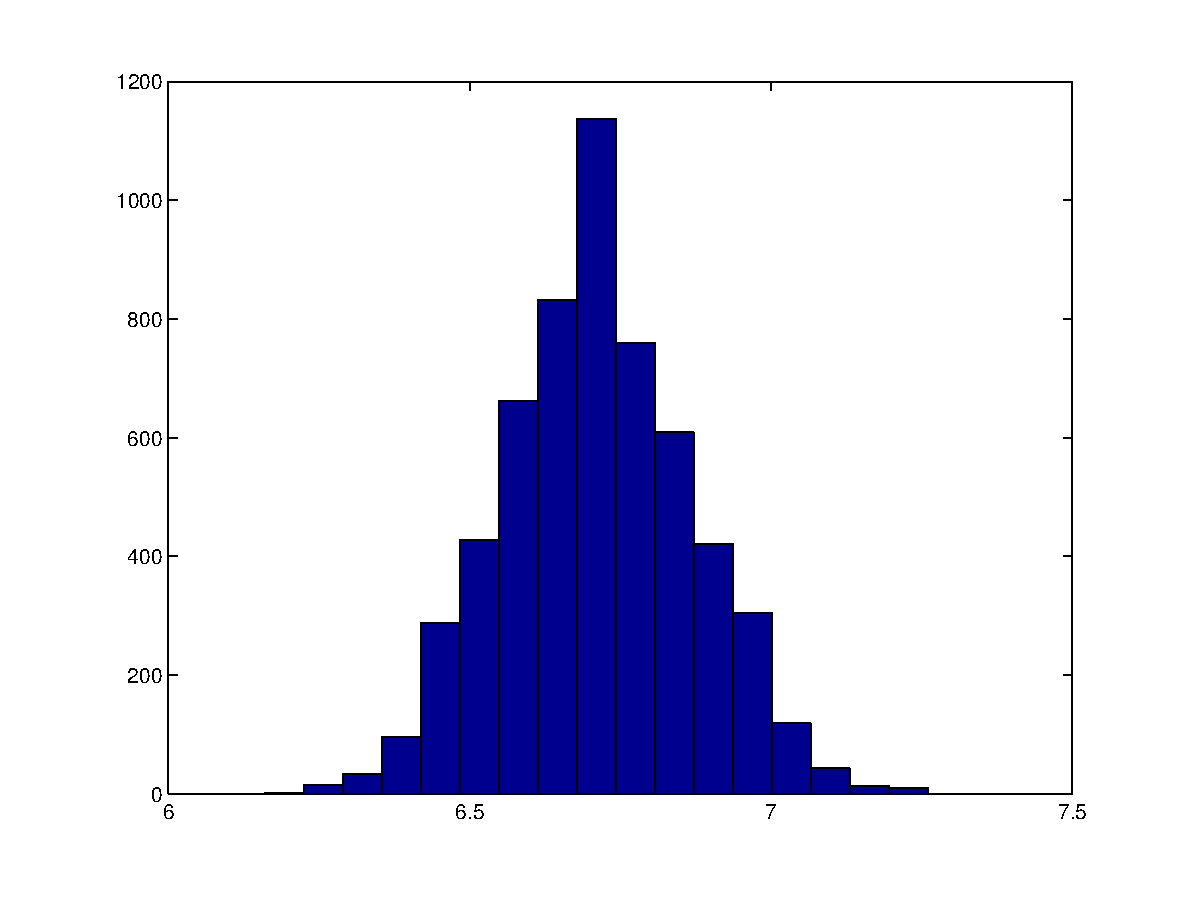
\epsfig{file=histrogramaConUnaTriangular.eps, scale=0.55}
\caption{Frecuencia de aparici\'on de los n\'umeros pseudo-aleatorio que representan a lo Per\'iodo}
\label{fig:histoTriangulo}
\end{figure} 
 
\section*{REFERENCIAS}
\textit{Diaz, "Simulaci\'on de Montecarlo", 2011} \\
\textit{Mathworks, "http://www.mathworks.com/help/techdoc/ref/ode45.html", 2011}
\end{document}


